\documentclass[10pt]{article}

% Include Theme
% Margins ----------------------------------------------------------------------

\usepackage[margin=1.25in]{geometry}

% AMS --------------------------------------------------------------------------

\usepackage{amsmath}
\usepackage{amsfonts}
\usepackage{amsthm}
\usepackage{graphicx}


% Line Spacing -----------------------------------------------------------------

\renewcommand{\baselinestretch}{1.5}


% Font -------------------------------------------------------------------------

\usepackage[T1]{fontenc}
\usepackage[default]{lato}
% \usepackage[utopia, varg]{newtxmath}
% \renewcommand{\rmdefault}{futs} % Utopia as text font 

% Small adjustments to text kerning
\usepackage{microtype}

% Remove annoying over-full box warnings
\vfuzz2pt 
\hfuzz2pt


% Tikz support -----------------------------------------------------------------

\usepackage{tikz}


% Color Palette ----------------------------------------------------------------

\usepackage{xcolor}

% https://www.materialpalette.com/colors
\definecolor{dark-maroon}{HTML}{5D0F0D}
\definecolor{navyblue}{HTML}{0A3044}

% https://www.viget.com/articles/color-contrast/
\definecolor{purple}{HTML}{5601A4}
\definecolor{navy}{HTML}{0D3D56}
\definecolor{ruby}{HTML}{9a2515}
\definecolor{alice}{HTML}{107895}
\definecolor{daisy}{HTML}{EBC944}
\definecolor{coral}{HTML}{F26D21}
\definecolor{kelly}{HTML}{829356}
\definecolor{cranberry}{HTML}{E64173}
\definecolor{jet}{HTML}{131516}
\definecolor{asher}{HTML}{555F61}
\definecolor{slate}{HTML}{314F4F}


% Hyperlinks -------------------------------------------------------------------

\usepackage{hyperref}
\hypersetup{
    colorlinks= true,
    citecolor= dark-maroon,
    linkcolor= dark-maroon,
    filecolor= dark-maroon,      
    urlcolor= dark-maroon,
}


% Citations --------------------------------------------------------------------

% note, natbib provides better hyperlinking
\usepackage{natbib}
\bibliographystyle{econ-aea}
% How to display multiple in \citet{}
\setcitestyle{comma,aysep={}}

% Define Theorems --------------------------------------------------------------

% Put proper spacing after Theorem #. 
\newtheoremstyle{spacing}
{}%          Space above, empty = `usual value'
{}%          Space below
% {\itshape}%  Body font
{}%  Body font
{}%          Indent amount (empty = no indent, \parindent = para indent)
{\bfseries\color{navyblue}}% Thm head font
{.\ }%         Punctuation after thm head
{2.5mm}%  Space after thm head: \newline = linebreak
{}%          Thm head spec

% note, theorem is the name that goes in \begin{} and Theorem is the name displayed as Theorem 1
\theoremstyle{spacing}
\newtheorem{theorem}{Theorem}
\newtheorem{proposition}{Proposition}
\newtheorem{assumption}{Assumption}
\newtheorem{remark}{Remark}
\newtheorem{example}{Example}


% Custom Math Definitions ------------------------------------------------------

\global\long\def\expec#1{\mathbb{E}\left[#1\right]}%
\newcommand{\condexpec}[2]{\mathbb{E}\left[#1 \ \vert \ #2\right]}
\global\long\def\prob#1{\mathbb{P}\left[#1\right]}%
\global\long\def\var#1{\mathrm{Var}\left[#1\right]}%
\global\long\def\cov#1{\mathrm{Cov}\left[#1\right]}%
\global\long\def\one{\mathbf{1}}%


% Titlepage --------------------------------------------------------------------

% \maketitle
\usepackage{titling}
\usepackage{setspace}

% title
\pretitle{\begin{spacing}{1}\begin{flushleft}\huge}
\posttitle{\end{flushleft}\end{spacing}\vspace{-5mm}}
% author, note don't use \and 
\preauthor{\begin{flushleft}\LARGE}
\postauthor{\end{flushleft}\vspace{-7.5mm}}
% date
\predate{\begin{flushleft}\Large\color{asher}}
\postdate{\end{flushleft}\vspace{-5mm}}

% Abstract
\renewenvironment{abstract}
 {\noindent\rule{\linewidth}{.5pt}\noindent}
 {\noindent\rule{\linewidth}{.5pt}}

% alternative abstract
% \renewenvironment{abstract}
% {
%   \centerline {\large \bfseries \scshape \color{navyblue} Abstract}
%   \begin{quote}
% }
% {\end{quote}}


% Section and Subsection Styling -----------------------------------------------

\usepackage[explicit]{titlesec}

\titleformat{\section}
  {\large \bf \color{navyblue}}
  {\thesection \,---}
  {0.25em}
  {#1}
  
\titleformat{\subsection}
  {\fontsize{11}{10}\it}
  {\thesubsection.}
  {1em}
  {#1}


% Footnote ---------------------------------------------------------------------

% Spacing between footnotes on same page
\addtolength{\footnotesep}{1mm}

% Space after footnote number
\let\oldfootnote\footnote
\renewcommand\footnote[1]{\oldfootnote{\ #1}}

% No footnote line
\renewcommand\footnoterule{}

% No supsercript in footer
\makeatletter
\renewcommand\@makefntext[1]{%
    \parindent 1em \noindent
    \hb@xt@1.8em{\hss\normalfont\@thefnmark.\hfill}#1
  }
\makeatother




% Enumerate/Itemize ------------------------------------------------------------

\usepackage{enumitem}
\setitemize{labelindent=0.5em,labelsep=0.25cm,leftmargin=*}
\setenumerate{labelindent=0.5em,labelsep=0.25cm,leftmargin=*}


% Table and Figure labelling ---------------------------------------------------

\usepackage{caption}

\DeclareCaptionLabelSeparator{threedash}{\,---\,}
\DeclareCaptionFont{navyblue}{\color{navyblue}}
\DeclareCaptionFont{jet}{\color{jet}}
\captionsetup[table]{format=plain, labelsep=threedash, font={navyblue, bf}}
\captionsetup[figure]{format=plain, labelsep=threedash, font={navyblue, bf}}

% Alternative: Left align captions
% \captionsetup[table]{labelfont=it, textfont={navyblue, bf}, labelsep=newline, justification=raggedright, singlelinecheck=off}
% \captionsetup[figure]{labelfont=it, textfont={navyblue, bf}, labelsep=newline, justification=raggedright, singlelinecheck=off}

% multifigure with \caption
% \begin{subfigure}\caption{} \end{subfigure}
\usepackage{subcaption}
\captionsetup[subfigure]{format=plain, font={jet, footnotesize, bf}}


% Tables -----------------------------------------------------------------------

% Fix \input with tables
% \input fails when \\ is at end of external .tex file
\makeatletter
\let\input\@@input
\makeatother

% Make tables/figures wider than \textwidth using:
% \begin{adjustbox}{width = 1.2\textwidth, center}
% \end{adjustbox}
\usepackage{adjustbox}

% Slighty more spacing between rows
\usepackage{array}
\renewcommand\arraystretch{1.25}

% Table with easy to use footnotes
% \begin{threeparttable}
%    \begin{tabular} ... \end{tabular}
%    \begin{tablenotes}
%        \item \textit{Notes.}
%    \end{tablenotes}  
% \end{threeparttable}
\usepackage[flushleft]{threeparttable}
\setlength\labelsep{0pt}

% \toprule, \cmidrule, \bottomrule
\usepackage{booktabs}

% If tables are too narrow, fill columns using:
% \begin{tabularx}{\linewidth}{cols}
% col-types: X - center, L - left, R -right
% If you want relative scale for columns: 
% >{\hsize=.8\hsize}X/L/R
\usepackage{tabularx}
\newcolumntype{L}{>{\raggedright\arraybackslash}X}
\newcolumntype{R}{>{\raggedleft\arraybackslash}X}
\newcolumntype{C}{>{\centering\arraybackslash}X}

% Landscape table 
% \begin{landscape} \pagestyle{lscaped} table... \end{landscsape}
% \usepackage{pdflscape} - rotates page left-side up in pdf
% \usepackage{lscape} - does not rotate page, only figure/table

\usepackage{pdflscape}

% For landscape, fix page number location
\usepackage{fancyhdr}
\fancypagestyle{lscaped}{%
    \fancyhf{}
    \renewcommand{\headrulewidth}{0pt}
    \textnormal
    \fancyfoot{%
        \tikz[remember picture,overlay]
        \node[outer sep=2.5cm,above,rotate=90] at (current page.east) {\thepage};
    }
}
  

% ------------------------------------------------------------------------------


% \maketitle info
\title{Difference-in-Differences with Geocoded Microdata}
\author{\href{https://kylebutts.com/}{Kyle Butts}\thanks{University of Colorado, Boulder. Email: \href{mailto:kyle.butts@colorado.edu}{kyle.butts@colorado.edu}.} % \ and Other Author}
}
\date{\today}

\newcommand{\dist}{\text{Dist}}

% pdf info
\hypersetup{pdftitle={Example Paper}, pdfauthor={Kyle Butts}}

\begin{document}

% Title Page -------------------------------------------------------------------
\maketitle

\begin{abstract}
    This paper formalizes a common approach for estimating effects of treatment at a specific location using geocoded microdata. This estimator compares units immediately next to treatment (an inner-ring) to units just slightly further away (an outer-ring). This paper formalizes the necessary assumptions to identify the average treatment effect among the effected units and illustrates potential pitfalls when these assumptions fail. Since one of these assumptions requires knowledge of exactly how far treatment effects are experienced, I propose a new method that relaxes this assumption and allows for non-parametric estimation using partitioning-based least squares developed in \citet{Cattaneo_Crump_Farrell_Feng_2019}. This method allows for researchers to estimate how treatment effects evolve over distance. Lastly, I illustrate the advantage of this method by revisiting the effects of increased crime risk on home values studied in \citet{Linden_Rockoff_2008}. 

    \par~\par\noindent
    JEL-Classification: C13, C14, C18
    \par\noindent
    Keywords: Spatial, Difference-in-Differences
    \par
\end{abstract}
\newpage

% Paper ------------------------------------------------------------------------

% ------------------------------------------------------------------------------
\section{Introduction}
% ------------------------------------------------------------------------------

The rise of microdata with precisely geocoded locations has allowed researchers to begin answering questions about the effects of some specific treatment at a very granular level. What are the effects of highly localized pollutants on child health? Does being within walking distance to a new bus stop improve labor market outcomes? How far do neighborhood shocks such as foreclosures or new construction spread? When treatment is located at a specific point in space, a standard method of evaluating the effects of the treatment is to compare units that are close to treatment to those slightly further away -- what I will label the `Ring method'. This paper fills a gap in the literature by formalizing the assumptions required for identification, highlighting potential pitfalls to the currently used estimator, and provides an improved estimator which requires fewer assumptions. 

The ring method is illustrated in \autoref{fig:example-id}. The center of the figure marks an x which represents the locatin of treatment, e.g. a foreclosed home. Units marked by circles are considered treated due to their proximity to the treatment location, units marked in triangles are considered control units, and then the remaining units are removed from the sample. The appeal of this identification strategy is that since the treated and control units are all very close in physical location, e.g. having access to the same labor market and consumptive amenities, the counterfactual outcomes will approximately be equal between both rings. The ring method compares average changes in outcomes between units in the inner treated ring and the outer control ring to form an estimate for the treatment effect. 

The first contribution of the paper is to fill a gap in the econometrics literature by formalizing the necessary assumptions for unbiased estimates of the average treatment effect on the affected units. The first assumption is the well understood parallel trends assumption for the treated and control units. This allows for average changes in the control units to estimate the counterfactual trend for the treated units.

% Figure: Example ID -----------------------------------------------------------

\begin{figure}[tb]
    \caption{Rings Method}
    \label{fig:example-id}

    \begin{adjustbox}{width = 0.4\textwidth, center}
        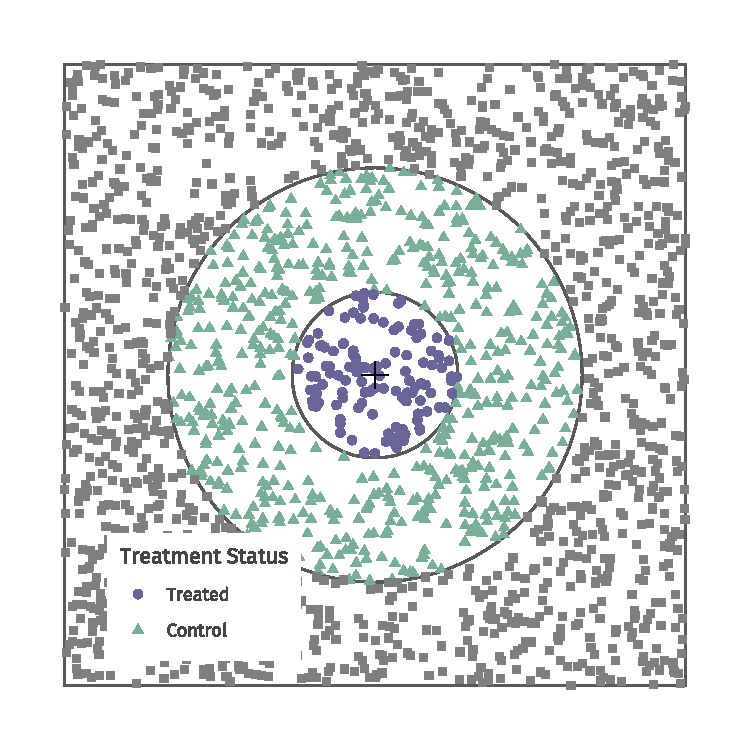
\includegraphics[width=\textwidth]{../../figures/example_id.pdf}
    \end{adjustbox}
\end{figure}

The second assumption reqires that the radius of the treated ring must be correctly specified as the maximum distance that experiences effects of treatment. If the treated ring is too narrow, then units in the control ring experience effects of treatment and the change among `control' units would no longer identify the counterfactual trend. On the other hand, if the treated ring is too wide, then the 0 treatment effect of some unaffected units are averaged into the change among `treated' units. Therefore results will be attenuated towards zero.\footnote{This is equivalent to randomly assigning treated status to a portion of control units in an experiment.}

Since this second assumption of how far treatment effects extend is difficult to know in most circumstances, I propose a method that replaces this assumption with a more mild assumption by using nonparametric partitioning-based least square regressions \citep{Cattaneo_Farrell_Feng_2019,Cattaneo_Crump_Farrell_Feng_2019}. My proposed methodology estimates the treatment effect curve rather than trying to estimate an average affect. There are many advantages to this approach. First, the new assumption required is much more mild as it only requires that treatment effects become zero somewhere between the distance of 0 and the control ring which does not have to be known by the researcher. Second, this approach allows researcher to get a more complete picture of how the intervention affects units at various distance rather than estimating an ``overall effect''. For example, potentially a new bus-stop creates costs to immediate neighbors while provides benefits for homes slightly further away. Estimation of the treatment effect curve can illustrate these different effects that the ``overall effect'' would mask over. Lastly, this approach allows visual evidence to plausibly validate the parallel trends assumption at the heart of this method, akin to the pre-trends test in event studies.

% ------------------------------------------------------------------------------
\subsection{Relation to Literature}
% ------------------------------------------------------------------------------




% ------------------------------------------------------------------------------
\section{Example of Problem}
% ------------------------------------------------------------------------------

To illustrate the methodological difficulties in this method, I present an illustriative example. Suppose that an overgrown empty lot in a high-poverty neighborhood is cleaned up by the city and the outcome of interest is home prices. The researcher observes a panel of home sales before and after the lot is cleaned. Cleaning up the lot causes home values to go up directly nearby and as you move away from the lot, the positive treatment effect will decay to zero effect at, say, 3/4 of a mile. Since treatment is targeted to the high poverty neighborhood, comparisons with other neighborhoods in the cities could be biased if the neighborhood home prices are on different trends. Hence, the researcher wants to look only at the homes in the immediate neighborhood.

% Figure: Example problem ------------------------------------------------------

\begin{figure}[tb]
    \caption{Example of Problems with Ad-Hoc Ring Selection}
    \label{fig:problems}

    \begin{adjustbox}{width = 1.1\textwidth, center}
        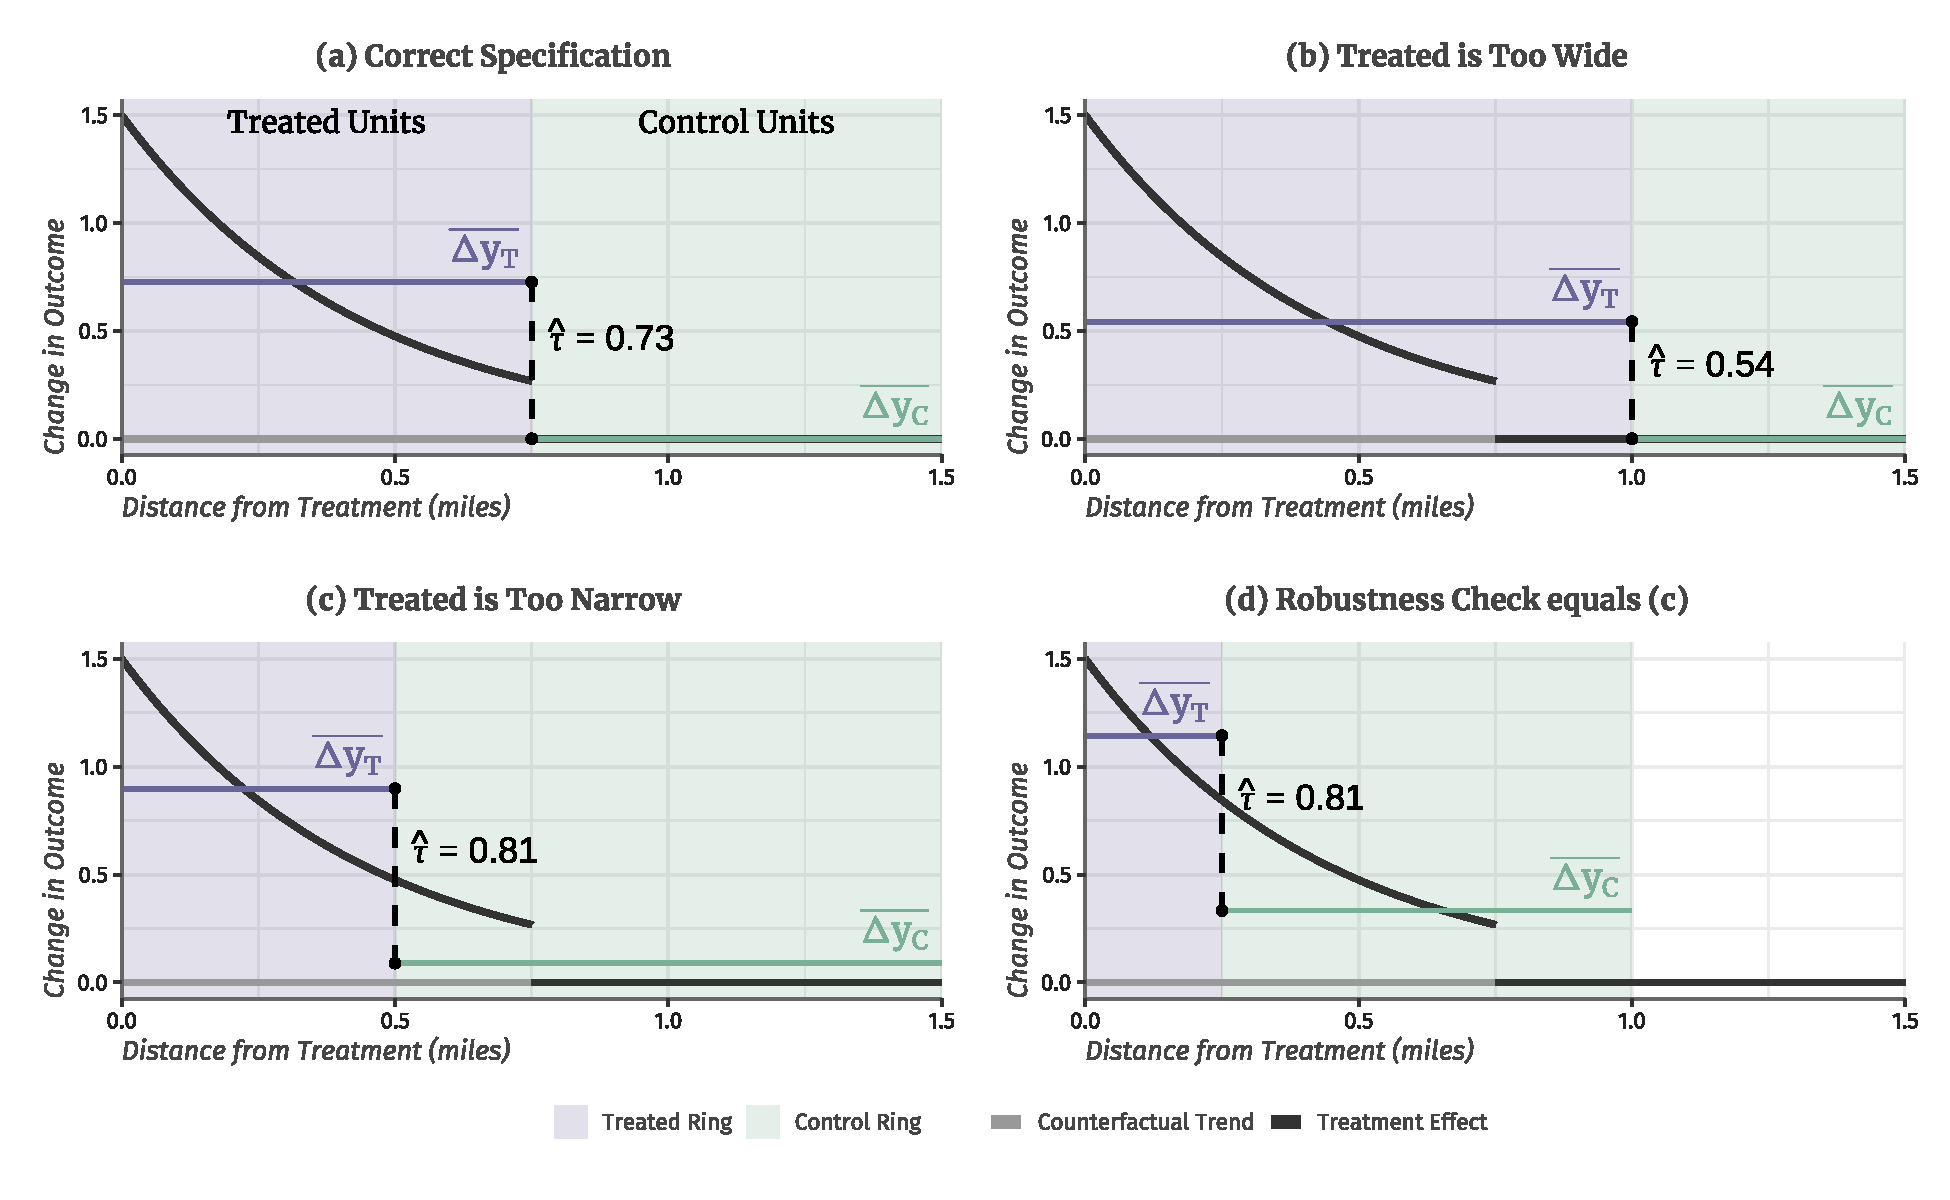
\includegraphics[width=\textwidth]{../../figures/example.pdf}
    \end{adjustbox}

    {\footnotesize \emph{Notes:} This figure shows an example of the ring method. The inner ring marks units considered `treated', the outer ring marks units considered `control' units, and the rest of the observations are removed from the sample. Then average changes in outcomes are compared between the treated and the control units to form a treatment effect estimate.}
\end{figure}

\autoref{fig:problems} shows a plot of simulated data from this example. The black line is treatment effect at different distances from the empty lot and the grey line is the trend in home values. In this simple example, counterfactual trends are assumed to be constant within 1.5 miles from the treated lot. Panel (a) of \autoref{fig:problems} shows the best-case scenario where the treated ring is correctly specified. The two horizontal lines show the average change in outcome in the treated ring and the control ring. The treatment effect estimate, $\hat{\tau}$, is the difference between these two averages. However, this singular number masks over a large amount of treatment effect heterogeneity with units very close to treatment having a treatment effect double that of $\hat{\tau}$ and units near 3/4 miles experience a treatment efffect half as large as $\hat{\tau}$. For this reason, even if a researcher identifies the correct average treatment effect, they are masking a lot of heterogeneity that is potentially interesting. Therefore, later in this paper I recommend non-parametrically estimating the treatment effect as a function of distance rather than using a single indicator. 

However, the researcher does not typically know the distance at which treatment effects stop. Panels (b) and (c) highlights how treatment effect estimates change with a change in ring distances. Panel (b) shows when the `treatment' ring is too wide. In this case, some of the units in the treatment ring receive no effect from treatment and therefore makes the average treament effect among units in the treatment ring smaller. Therefore when the treated ring is too large, the estimated treatment effect is too small.

Panel (c) of \autoref{fig:problems} shows the opposite case, where the treated ring is too narrow. In this case, there are some units in the `control' ring that experience treatment effects. Hence, the average change in outcome among the control unit is too large. This does not, though, decrease the treatment effect as you may suspect. Since the treatment effect decays with distance, the average change in outcome among the more narrow `treatment' ring is larger than the correct specification. The estimated treatment effect in this case grows, but it is not clear more generally whether the treatment effect will increase or decrease. 

This estimation strategy requires researchers to know the exact distance at which treatment effects become zero. Since this is a very demanding assumption, I propose an improved estimator in Section \ref{sec:lspartition} that relaxes this assumption. 

Often times, researchers try multiple sets of rings and if the estimated effect remains similar across specifications, they assume the results are `robust'. Panel (d) of \autoref{fig:problems} shows an example of why this a problem. If Panel (c) was the researchers' original specification and Panel (d) was run as a robustness check, then the researcher would be quite confident in their results even though the estimate is too large in both cases. 



% ------------------------------------------------------------------------------
\section{Theory}
% ------------------------------------------------------------------------------

Now, I develop econometric theory to formalize the intuition developed in the previous section. A researcher observes panel data of a random sample of units $i$ at times $t = 0, 1$ located in space at point $\theta_i = (x_i, y_i)$. Treatment occurs at a location $\bar{\theta} = (\bar{x}, \bar{y})$ between periods. Therefore, units differ in their distance to treatment, defined by $\dist_i \equiv \sqrt{(x_i - \bar{x})^2 + (y_i - \bar{y})^2}$ with a distribution function $F$. Since treatment location is often chosen strategically, potential outcomes will have to reflect the fact that trends can change with distance to treatment. Outcomes are given by 
\[ 
    Y_{it} = \tau(\dist_i) \one_{t = 1} + \mu_i + \lambda(\dist_i) \one_{t=1} + \varepsilon_{it},    
\]
where $\tau(\dist)$ is the treatment effect curve at different distances, $\mu_i$ is unit-specific time-invariant factors, and $\lambda(\dist)$ is the counterfactual trend at different distances from treatment. Since we include the $\lambda$ term, without loss of generality we assume that the error term $\varepsilon_{it}$ is uncorrelated with distance to treatment. Researchers are trying to identify the average treatment effect on units experiencing treatment effects, i.e. $\bar{\tau} = \condexpec{\tau(\dist)}{\tau(\dist) > 0}$ where expectations are with respect to the distribution of distances.

% \begin{assumption}[Random Sampling]
%     The observed data consists of $\{ Y_{i1}, Y_{i0}, \dist_{i}\}$ which is independent and identically distributed.
% \end{assumption}

Taking first-differences of our model, we have $\Delta Y_{it} = \tau(\dist_i) + \lambda(\dist_i) + \Delta \varepsilon_{it}$. It is clear that $\tau(\dist_i)$ and $\lambda(\dist_i)$ are not seperately identified unless additional assumptions are imposed. Often times researchers claim that counterfactual trends likely evolve smoothly over distance, so that $\lambda(\dist_i)$ is approximately constant within a certain distance from treatment. This is formalized in the context of our outcome model by the following assumption. 

\begin{assumption}[Local Parallel Trends]\label{assum:parallel}
    For a distance $\bar{d}$, we say that local parallel trends hold if for all positive $d, d' \leq \bar{d}$, then $\lambda(d) = \lambda(d')$.
\end{assumption}

This assumption requires that, in the absence of treatment, outcomes would evolve the same at every distance from treatment within a certain maximum distance, $\bar{d}$. If this assumption holds for some $d_c$, then our first-difference equation can be simplified to $\Delta Y_{it} = \tau(\dist_i) + \lambda + \Delta \varepsilon_{it}$ where $\lambda$ is some constant. Therefore, the treatment effect curve $\tau(\dist_i)$ is identifiable up to a constant under Assumption \ref{assum:parallel}. To identify $\tau(\dist_i)$ seperately from the constant, researchers will often claim that treatment effects stop occuring before $\bar{d}$ and therefore there are valid `control units` in the sample. This is formalized in the following assumption. 

\begin{assumption}[Correct $d_t$]\label{assum:dt}
    A distance $d_t$ satisfies this assumption if (i) for all $d \leq d_t$, $\tau(d) > 0$ and for all $d > d_t$, $\tau(d) = 0$ and (ii) $F(\bar{d}) - F(\bar{d_t}) > 0$
\end{assumption}


The second part of this assumption just requires that there are observation in the control ring.

The `ring method' is the following procedure. Researchers select a pair of distances $d_t < d_c$ which define the ``treated'' and ``control'' groups. These groups are defined by $\mathcal{D}_t \equiv \{ i : 0 < \dist_i \leq d_t \}$ and $\mathcal{D}_c \equiv \{ i : d_t < \dist_i \leq d_c \}$. On the subsample of observations defined by $\mathcal{D} \equiv \mathcal{D}_t \cup \mathcal{D}_c$, they run the following specification:
\begin{equation}\label{eq:ring_method}
    \Delta Y_{it} = \beta_0 + \beta_1 \one_{i \in \mathcal{D}_t} + u_{it}.
\end{equation}

From our potential outcome framework and standard results for regressions involving only indicators, we have the following proposition.\footnote{A similar derivation of part (i) is found in \citet{Sullivan_2017}.}

\begin{proposition}[Decomposition of Ring Estimate]\label{prop:ring_decomp}     
    \par~\par
    \begin{enumerate}
        \item[(i)] The estimate of $\beta_1$ in (\ref{eq:ring_method}) has the following expectation:
        \[
            \expec{\hat{\beta}_1} = 
            \underbrace{\condexpec{\tau(\dist)}{\mathcal{D}_t} - \condexpec{\tau(\dist)}{\mathcal{D}_c} }_{\text{Difference in Treatment Effect}} 
            + \underbrace{\condexpec{\lambda(\dist)}{\mathcal{D}_t} - \condexpec{\lambda(\dist)}{\mathcal{D}_c} }_{\text{Difference in Trends}}.
        \]
        
        \item[(ii)] More, if $d_c$ satisfies Assumption \ref{assum:parallel}, then
        \[ 
            \expec{\hat{\beta}_1} = 
            \underbrace{\condexpec{\tau(\dist)}{\mathcal{D}_t} - \condexpec{\tau(\dist)}{\mathcal{D}_c} }_{\text{Difference in Treatment Effect}}.
        \] 
    
        \item[(iii)] If $d_c$ satisfies Assumption \ref{assum:parallel} and $d_t$ satisfies Assumption \ref{assum:dt}, then
        \[ 
            \expec{\hat{\beta}_1} = \bar{\tau}.
        \]
    \end{enumerate}
    
    
\end{proposition}

Part (i) of this proposition shows that the `treatment effect' estimate is the sum of two differences. The first difference is the difference in average treatment effect among units in the treated ring and units in the control ring. If some units in the control group experience effects from treatment, the average of these effects will be subtracted from the estimate. The second difference is the difference in counterfactual trends between the treated and control rings. Since treatment can be targeted, the treated ring could be on a different trend than units further away. This difference in counterfactual trends is not seperately identifiable from the difference in average treatment effects unless Assumption \ref{assum:parallel} is satisfied. 

Part (ii) says that if $d_c$ satisfies Assumption \ref{assum:parallel}, then the counterfactual trend from part (i) is equal to 0. As discussed above, the decomposition in part (ii) of Proposition \ref{prop:ring_decomp} is not necessarily unbiased estimate for $\bar{\tau}$. First, if $d_t$ is \emph{too wide}, then $\mathcal{D}_t$ contain units that are not affected by treatment. In this case, $\condexpec{\tau(\dist)}{\mathcal{D}_t}$ will be smaller than $\bar{\tau}$ while $\condexpec{\tau(\dist)}{\mathcal{D}_c}$ would be equal to zero. Therefore, $\hat{\beta}_1$ will be biased towards zero if $d_t$ is too wide. Second, if $d_t$ is {too narrow} then the $\mathcal{D}_c$ will contain units that experience treatment effects. It is not clear in this case, though, if $\hat{\beta}_1$ will grow or shrink without knowledge of the $\tau(\dist)$ curve, but typically $\hat{\beta}_1$ will not be an unbiased estimate for $\bar{\tau}$. See the previous section for an example. 

Part (iii) of Proposition \ref{prop:ring_decomp} shows that if $d_t$ is correctly specified as the maximum distance that receives treatment effect, then $\hat{\beta}_1$ will be an unbiased estimate for the average treatment effect among the units affected by treatment. However, Assumption \ref{assum:dt} is a very demanding assumption and unlikely to be known by the researcher unless there are a priori theory dictating $d_t$.\footnote{As an example of a priori theory dictating $d_t$, \citet{Currie_Davis_Greenstone_Walker_2015} uses results from chemical studies on the maximum spread of local pollutants and \citet{Marcus_2021} use the plume length of petroleum smoke.} The following section will improve estimation by allowing non-parametric identification of the entire $\tau(\dist)$ function. An estimate of $\tau(\dist)$ can then be numerically integrated to for an estimate of $\bar{\tau}$.

% ------------------------------------------------------------------------------
\subsection{Estimation of $\tau(\dist)$}\label{sec:lspartition}
% ------------------------------------------------------------------------------

In this section, I propose an estimation strategy that non-parametrically identifies the treatment effect curve $\tau(\dist_i)$. To do this, I use partitioning-based least squares estimation and inference methods developed in \citet{Cattaneo_Farrell_Feng_2019,Cattaneo_Crump_Farrell_Feng_2019}. Partition based estimators seperate the support of a covariate $x$, such as $\text{\dist}$, into a set of quantile-spaced rings (e.g. 0-25th percentiles of $X$, 25-50th percentiles, 50-75th, 75-100th) and estimate a polynomial within each interval. In this way, any function can be approximated nonparametrically as the number of intervals and the degree of the polynomial increase asymptotically. 

For a given partition based on quantiles of the data $\{ \mathcal{D}_1, \dots, \mathcal{D}_k \} \equiv \mathcal{D}$, we will estimate the conditional average of $\Delta Y_{it}$ for each interval $\mathcal{D}_i$. These averages are defined as 
\[
    \overline{\Delta Y}_j \equiv \sum_{i \in \mathcal{D}_j} \Delta Y_{it} 
\]
This will form our estimate $\tau(\dist_i) + \lambda$ under local parallel trends, Assumption \ref{assum:parallel}. To remove $\lambda$, we require an Assumption like \ref{assum:dt}.

\begin{assumption}[$d_t$ is within $\bar{d}$]\label{assum:dt_weak}
    A distance $\bar{d}$ satisfies this assumption if there is a distance $d_t$ with $0 < d_t < \bar{d}$ such that (i) Assumption \ref{assum:dt} holds and (ii) $F(\bar{d}) - F(d_t) > 0$.
\end{assumption}

Under Assumptions \ref{assum:parallel} and \ref{assum:dt_weak}, the mean within the last ring $\mathcal{D}_k$ will estimate $\lambda$ as the number of bins $k \to \infty$. The reason for this is simple, as $k \to \infty$, the last bin will have the left end-point $d > d_t$ and therefore $\tau(\dist) = 0$ in $\mathcal{D}_k$. Therefore, estimates of $\tau(\dist_i)$ can be formed for each interval as $\bar{\tau}_j \equiv \overline{\Delta Y}_j - \overline{\Delta Y}_k$. The results of \citet{Cattaneo_Crump_Farrell_Feng_2019} show the large-sample asymptotics of the estimates $\bar{\tau}_j$ which allow valid inference to be performed on these estimates.  

% ------------------------------------------------------------------------------
\newpage~\bibliography{references.bib}
% ------------------------------------------------------------------------------


\end{document}